%%%%%%%%%%%%%%%%%%%%%%%%%%%%%%%%%%%%%%%%%%%%%%%%%%%%%%%%%%%%%%%%%%%%%%%%%%%%%%%%
%2345678901234567890123456789012345678901234567890123456789012345678901234567890
%        1         2         3         4         5         6         7         8

\documentclass[letterpaper, 10 pt, conference]{ieeeconf}  % Comment this line out
                                                          % if you need a4paper
%\documentclass[a4paper, 10pt, conference]{ieeeconf}      % Use this line for a4
                                                          % paper

\IEEEoverridecommandlockouts                              % This command is only
                                                          % needed if you want to
                                                          % use the \thanks command
\overrideIEEEmargins
% See the \addtolength command later in the file to balance the column lengths
% on the last page of the document

\usepackage{cite}
\usepackage[pdftex]{graphicx}
\graphicspath{{../pdf/}{../jpeg/}}
\DeclareGraphicsExtensions{.pdf,.jpeg,.png,.eps}
\usepackage{epstopdf}
\usepackage[cmex10]{amsmath}
\usepackage{subfig}
\usepackage{dblfloatfix}
\usepackage{color}
\usepackage{amsmath}

% The following packages can be found on http:\\www.ctan.org
%\usepackage{graphics} % for pdf, bitmapped graphics files
%\usepackage{epsfig} % for postscript graphics files
%\usepackage{mathptmx} % assumes new font selection scheme installed
%\usepackage{times} % assumes new font selection scheme installed
%\usepackage{amsmath} % assumes amsmath package installed
%\usepackage{amssymb}  % assumes amsmath package installed

%
% paper title
% can use linebreaks \\ within to get better formatting as desired
\title{\LARGE \bf
Stabilizing a Quadruped robot locomotion\\ using a 2 Degree of Freedome Tail}


%\author{ \parbox{3 in}{\centering Huibert Kwakernaak*
%         \thanks{*Use the $\backslash$thanks command to put information here}\\
%         Faculty of Electrical Engineering, Mathematics and Computer Science\\
%         University of Twente\\
%         7500 AE Enschede, The Netherlands\\
%         {\tt\small h.kwakernaak@autsubmit.com}}
%         \hspace*{ 0.5 in}
%         \parbox{3 in}{ \centering Pradeep Misra**
%         \thanks{**The footnote marks may be inserted manually}\\
%        Department of Electrical Engineering \\
%         Wright State University\\
%         Dayton, OH 45435, USA\\
%         {\tt\small pmisra@cs.wright.edu}}
%}

%\author{Huibert Kwakernaak$^{1}$ and Pradeep Misra$^{2}$% <-this % stops a space
%\thanks{*This work was not supported by any organization}% <-this % stops a space
%\thanks{$^{1}$H. Kwakernaak is with Faculty of Electrical Engineering, Mathematics and Computer Science,
%        University of Twente, 7500 AE Enschede, The Netherlands
%        {\tt\small h.kwakernaak at papercept.net}}%
%\thanks{$^{2}$P. Misra is with the Department of Electrical Engineering, Wright State University,
%        Dayton, OH 45435, USA
%        {\tt\small p.misra at ieee.org}}%
%}

% author names and affiliations
% use a multiple column layout for up to three different
% affiliations

\author{Alan Mutka, Matko Orsag, and Zdenko Kovacic% <-this % stops a space
\thanks{The work presented in this paper was carried out within the project “Integrated Control of Robotic Systems in Complex Environments“ that is supported by a grant from the Croatian Ministry of Science, Education and Sports.}% <-this % stops a space
\thanks{A. Mutka, M. Orsag and Z. Kovacic are with the Laboratory for Robotics and Intelligent Control Systems, Universirty of Zagreb, Croatia, {\tt\small\{amutka, morsag, zkovacic\}{@}fer.hr}}
}

\begin{document}

\maketitle
\thispagestyle{empty}
\pagestyle{empty}

%%%%%%%%%%%%%%%%%%%%%%%%%%%%%%%%%%%%%%%
% Abstract
\begin{abstract}
%\boldmath
This paper presents the use of a tail for quadruped robot locomotion in order to apply additional forces/torques to stabilize the motion during flight phases in which the robot has no contact with the ground. The paper presents a Denavit-Hartenberg parameterization based kinematics of a two degree of freedom tail combined with a Newton-Euler based dynamic model. Impedance based leg control simplifies the leg motion so that it can be modeled as a dampened spring system. Finally, a recursive algorithm that moves the tail in order to balance the robot is proposed. A realistic model of the robot is built in Open Dynamic Engine environment and is used to conduct a series of tests proving the effectiveness of the proposed algorithm.
%Compared to autonomous ground vehicles, UAVs (unmanned aerial vehicles) have significant mobility advantages and the potential to operate in otherwise unreachable locations. Micro UAVs still suffer from one major drawback: they do not have the necessary payload capabilities to support high performance arms. This paper, however, investigates the key challenges in controlling a mobile manipulating UAV using a commercially available aircraft and a light-weight prototype 3-arm manipulator. Because of the overall instability of rotorcraft, we use a motion capture system to build an efficient autopilot. Our results indicate that we can accurately model and control our prototype system given significant disturbances when both moving the manipulators and interacting with the ground.
\end{abstract}

% IEEEtran.cls defaults to using nonbold math in the Abstract.
% This preserves the distinction between vectors and scalars. However,
% if the conference you are submitting to favors bold math in the abstract,
% then you can use LaTeX's standard command \boldmath at the very start
% of the abstract to achieve this. Many IEEE journals/conferences frown on
% math in the abstract anyway.

% no keywords


%%%%%%%%%%%%%%%%%%%%%%%%%%%%%%%%%%%%%%%
% Introduction
\section{Introduction}\label{sec:introduction}
% no \IEEEPARstart

Animals utilize tails in a variety of ways: to propel themselves through water; to help improve locomotion and balance; and some even use their tails for hanging on branches or for grasping trees. Balance control while running and hopping, or while gliding and climbing are just few examples of how a tail can help animals to realize robust locomotion \cite{Thomas:Nature2012}. The use of a tail for dynamic stabilization has been reported in the case of dinosaurs, lizards, cats, primates and even humans \cite{ostrom1969osteology,PijnappelsSringer,Walker199841,JusufiIOP2010}. One of the challenges in the design of biologically inspired robot systems is studying phenomena in natural systems and extracting basic knowledge for building similar technical systems. This does not mean only mimicking the nature, but also searching for innovative solutions. One such challenge is to add a tail mechanism to a walking robot so that it improves robot locomotion in a similar way as an animal's tail would do. 
 
A tail can balance the robot's body in both static and dynamic sense. The main technique of using a tail as a dynamic stabilizer for quadruped robot locomotion is to apply additional forces/torques on its body. Uniroo \cite{zeglin1991uniroo} is one of the first robots which uses a single degree of freedom active tail to maintain constant body pitch with the purpose of emulating a hopping kangaroo. Another active tail stabilization case presented in \cite{conf/iros/Chang-SiuLTF11} uses a tail on a wheeled car as a means for robust maneuvering on uneven terrain and stable pitch control by applying the principle of conservation of the momentum. The MIT Cheetah robot \cite{DBLP:conf/iros/BriggsLHK12} uses a tail to improve robot's running capabilities and perform runs up to 30 mph. Additionally, the authors analyze several other artificial mechanisms which can be used for exerting non-contact forces/torques like a reaction wheel, reaction mass, thrusters etc. In \cite{PullinICRA12}, Pullin et all compared the use of a tail to classical differential drive steering for different surface conditions on a crawling mobile robot OctoRoACH. They showed how a tail could be used when rapid turning or evasive maneuvers are required under low friction surface conditions. Learning from aerial robots, one can apply the techniques used in \cite{Korpela2013ICRA,Orsag2012JINT} to model the dynamics of inertial appendages and the impact they have on the underlying robot body. This paper however, wishes to address an alternative use for a tail, its static balancing capabilities. A tail is envisioned here as a counterweight capable of shifting its center of mass so as to balance effectively the robot body.
 
\begin{figure}
                \centering
                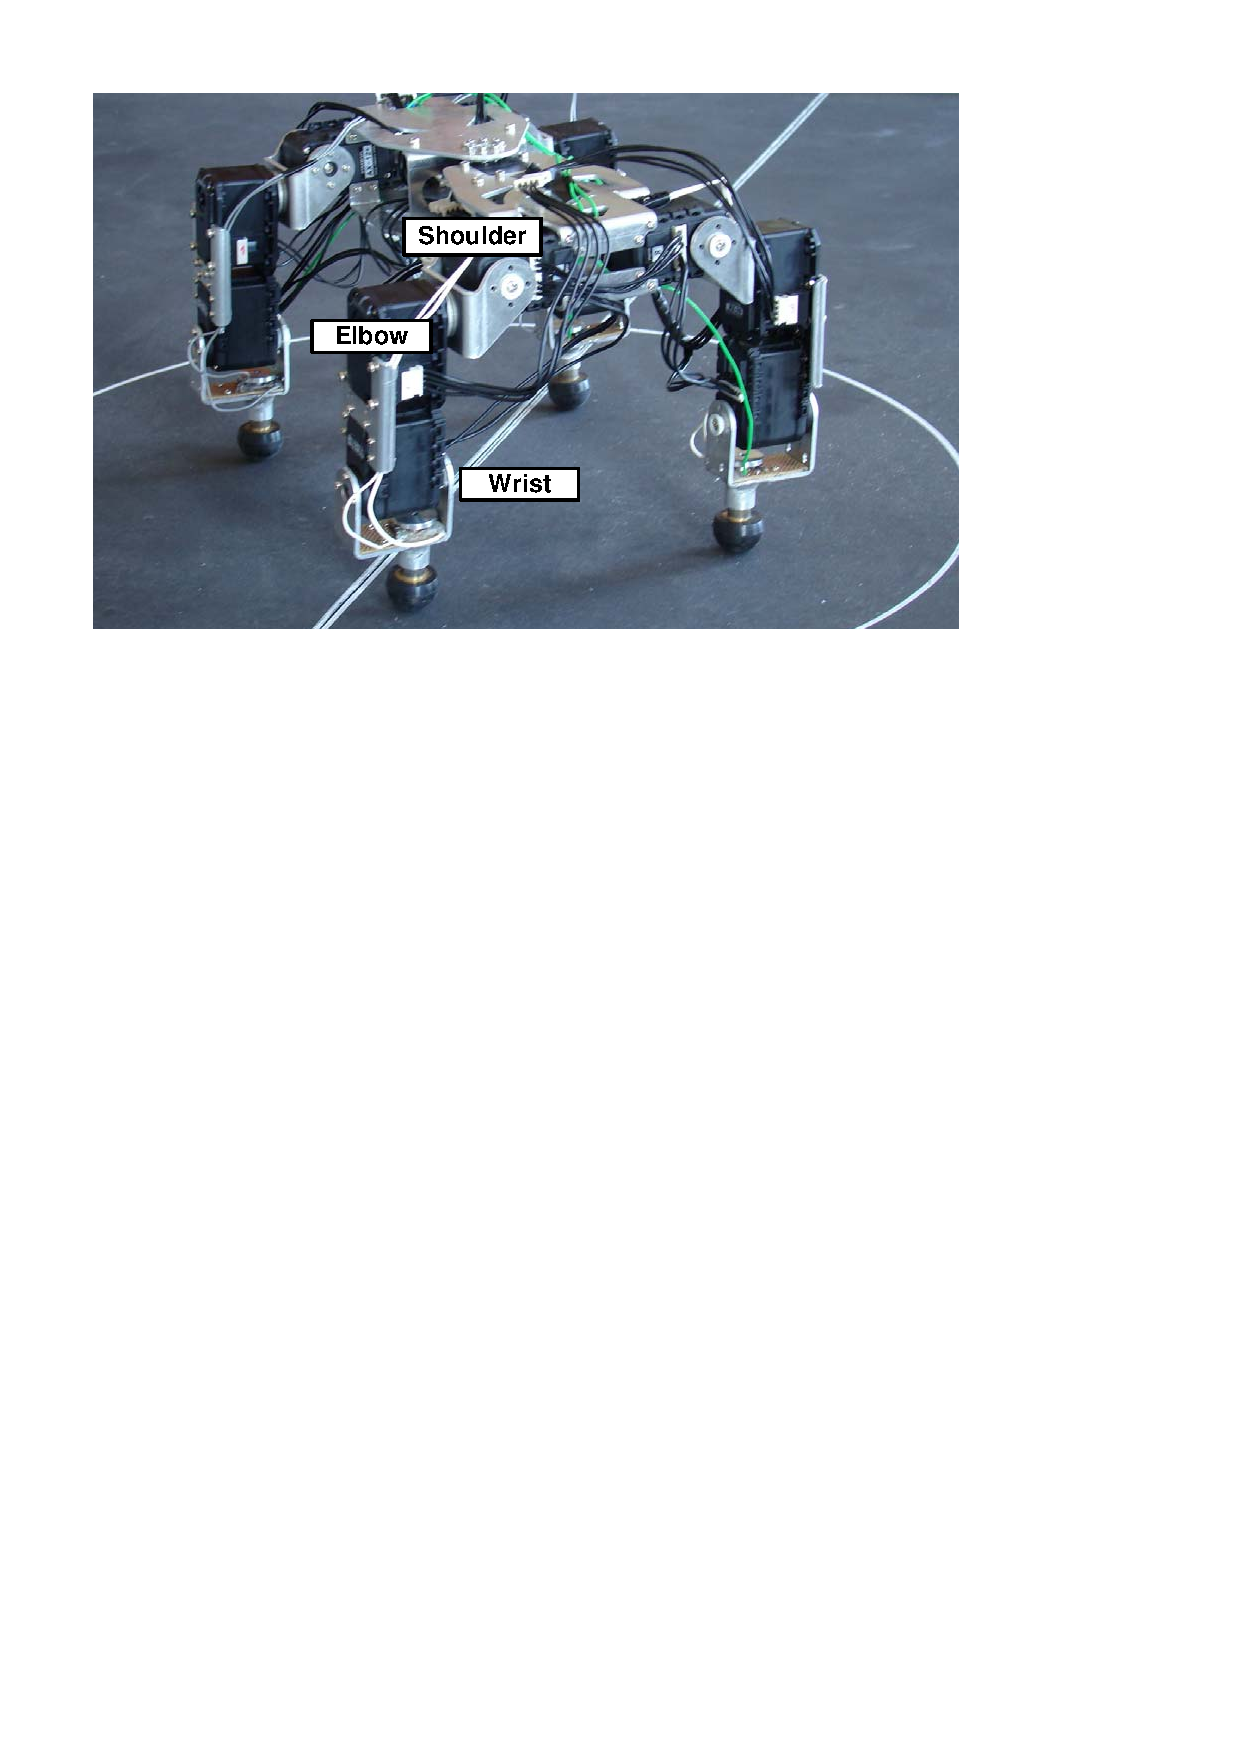
\includegraphics[width=75mm]{./pictures/Dynarobin_introduction_image.pdf}
                \caption{A quadruped robot Dynarobin \cite{DBLP:conf/IEEEcca/MutkaPRK12}}
                \label{fig:Dynarobin}
\end{figure}
 
Inspired by the agility of human and animal locomotion, over the last few decades the number of research groups presented numerous robot leg designs, and the associated modeling and control \cite{CambridgeJournals:1345088}. The predominant method for the modeling of quadruped locomotion gaits like walking, running, trotting, and bouncing is a spring-mass model\cite{Blickhan01}. This paper postulates that a single leg, hopping locomotion can also be described with a spring-mass model. In order to obtain a compliant robot leg behavior, impedance control is used to emulate a virtual spring-mass system \cite{Havoutis01}. By attaching four legs to one central body complex dynamic problems arise. In order to provide a stable quadruped hopping sequence a lot of parameters need to be observed: mass distribution, active and passive leg stiffness, ground stiffness, etc. This paper investigates how to improve locomotion stability of a dynamical system composed of four spring-masses by using a tail-like inertial appendage.
 
In Section \ref{sec:MathModel} a mathematical model of a quadruped robot Dynarobin (Fig. \ref{fig:Dynarobin}) together with a kinematic and a dynamic model of the tail is introduced. A single leg dynamics is modeled to mimic the behavior of an active spring-mass system. Building upon the results from Section \ref{sec:MathModel}, a recursive balancing algorithm is introduced in Section \ref{sec:Algorithm}. The algorithm is tested in the simulation environment which is described in Section \ref{sec:simulation}, along with the simulation results.




% Some research uses advanced variable stiffnes leg design %\cite{Hurst_2004_4785}\cite{Galloway}\cite{Jun:2009:DSV:1703775.1704089} which allows robot to run over a large variety %of terrains while adjusting their leg stiffness. All this research suggests that quadrupedal robot can be dynamically 5modeled as mass supported on four spring legs as shown in fig. 




%%%%%%%%%%%%%%%%%%%%%%%%%%%%%%%%%%%%%%%

%%%%%%%%%%%%%%%%%%%%%%%%%%%%%%%%%%%%%%%%%%%%%%%%%%%%%%%%%%%%%%%%%%%%%%%%%%%%%%%%

\addtolength{\textheight}{-4cm}   % This command serves to balance the column lengths
                                  % on the last page of the document manually. It shortens
                                  % the textheight of the last page by a suitable amount.
                                  % This command does not take effect until the next page
                                  % so it should come on the page before the last. Make
                                  % sure that you do not shorten the textheight too much.

%%%%%%%%%%%%%%%%%%%%%%%%%%%%%%%%%%%%%%%%%%%%%%%%%%%%%%%%%%%%%%%%%%%%%%%%%%%%%%%%

\bibliographystyle{bibliography/IEEEtran}
\bibliography{bibliography/IEEEabrv,bibliography/bibliography}

\end{document}
